\documentclass{article}

% NeurIPS 2025 formatting
%\usepackage{neurips_2025}
\usepackage[preprint]{neurips_2025}

% Additional packages
\usepackage[utf8]{inputenc}
\usepackage{amsmath,amssymb,amsfonts,amsthm}
\usepackage{hyperref}
\usepackage{enumitem}
\usepackage{geometry}
\usepackage{booktabs}
\usepackage{microtype}
\usepackage{xcolor}
\usepackage{tikz}
\usetikzlibrary{arrows.meta,positioning,fit,backgrounds,calc}


%%%% Macros
\newcommand{\Loss}{\mathcal{L}}
\newcommand{\R}{\mathbb{R}}
\newcommand{\E}{\mathbb{E}}
\newcommand{\He}{\mathrm{He}}

%%%% Theorem environments
\newtheorem{definition}{Definition}[section]
\newtheorem{lemma}{Lemma}[section]
\newtheorem{proposition}{Proposition}[section]
\newtheorem{corollary}{Corollary}[section]
\newtheorem{remark}{Remark}[section]

\title{Barriers for Learning in an Evolving World: \\a Mathematical Understanding of Loss of Plasticity}

\author{%
  Amir Joudaki$^{1}$ \And
  Giulia Lanzillotta$^{1}$ \And
  Mohammad Samragh Razlighi$^{2}$ \And
  Iman Mirzadeh$^{2}$ \And
  Thomas Hofmann$^{1}$ \And
  Mehrdad Farajtabar$^{2}$ \And
  Fartash Faghri$^{2}$ \And
  \vspace{-20pt}
  \\
  $^{1}$ETH Zürich
  $^{2}$Apple \\
  \texttt{\{amir.joudaki, giulia.lanzillotta, thomas.hofmann\}@inf.ethz.ch} \\
  \texttt{\{fartash, m\_farajtabar, imirzadeh, m\_samraghrazlighi\}@apple.com}
}

\begin{document}
\maketitle

\begin{abstract}
According to Richard~Sutton, standard deep models trained with back‑propagation excel in the classic two‑phase paradigm: a long training phase on a mostly stationary data set, followed by frozen (or minimally fine‑tuned) deployment.  
Over extended interaction with non‑stationary environments, however, the very same optimisation process that created powerful representations gradually destroys the network's ability to continue learning.  
Sutton calls this phenomenon \emph{loss of plasticity}.  
This paper takes a first‑principles look at why gradient‑based models lose plasticity, offering
a definition based on dynamical‑system language,  
two general mechanisms—frozen units and cloned‑unit manifolds—that provably trap gradient trajectories, and  
conditions under which perturbations or architectural choices can prevent or undo the collapse.  
The resulting theory unifies several strands of ideas within a single mathematical framework. These results show a stark contrast, where properties such as low rank or simplicity bias are desirable in the two-phase learning regime, but lead to loss of plasticity. Thus, we consolidate key propositions of Sutton about barriers of learning continuously and point to several avenues for future research to overcome these barriers. 
\end{abstract}

\section{Introduction}
Back‑propagation's success rests on two tacit assumptions:
\begin{enumerate}
    \item \textbf{Stationarity.}  Training and deployment distributions are identical, so a network need not adapt after its weights are set.
    \item \textbf{One‑shot randomness.}  A single random initialisation injects diversity; thereafter weights specialise but are never refreshed.
\end{enumerate}
When an \emph{agent} must act in a world whose dynamics or task distribution keeps changing, those assumptions fail.  
Empirically, deep networks subjected to long sequences of tasks or slowly drifting data eventually learn no better than a shallow linear model.  
Typical symptoms are:
\begin{itemize}[nosep]
    \item Explosive weight magnitudes and saturated activations,
    \item "dead" ReLUs whose upstream parameters stop moving,
    \item collapsing effective rank of hidden representations,
    \item attention heads or filters that cease to contribute.
\end{itemize}
Sutton argues that such failures stem from back‑propagation itself: the algorithm is optimised for transient, single‑task learning; its ability to explore parameter space relies on the once‑only random seed, which is gradually forgotten. 

\paragraph{Goal of this paper.}
We revisit gradient descent and back‑propagation from scratch, asking:

\begin{quote}
\emph{What structural features of gradient flow inevitably give rise to loss of plasticity, and how might we design algorithms or architectures that stay plastic forever?}
\end{quote}

The central proposition of this work is that low rank representations are at the heart of loss of plasticity. While low-rank representations are known to improve accuracy on two-phased training system, as they reduce the effective number of parameters, they also make the network prone to loss of plasticity, as they reduce its effective features. 

\section{Preliminaries}
\label{sec:framework}

Let $\theta\in\Theta\subseteq\R^p$ denote the parameters of a neural network trained on stream~$\{(x_t,y_t)\}_{t\ge0}$ via gradient descent (or its stochastic variants).  Denote the loss $\Loss(\theta)$ and the continuous‑time gradient flow
\begin{equation}
    \frac{d\theta(t)}{dt} \;=\; -\nabla_\theta\Loss\bigl(\theta(t)\bigr).
\end{equation}

\begin{definition}[Loss of plasticity manifold]
\label{def:lop}
A smooth sub‑manifold $\mathcal{M}\subset\Theta$ induces loss of plasticity if
\begin{enumerate}[label=(\alph*)]
    \item \textbf{Tangency:} $\nabla_\theta\Loss(\theta)\in T_\theta\mathcal{M}$ for all $\theta\in\mathcal{M}$, where $T_\theta\mathcal{M}$ is the tangent space.
    \item \textbf{Stability type:} Let $N_\theta\mathcal{M}$ be the normal space.  \vspace{-4pt}
        \begin{align}
        \text{Stable:}\; &\forall v\in N_\theta\mathcal{M}\setminus\{0\}: v^\top\nabla_\theta^2\Loss(\theta)v > 0; \\
        \text{Unstable:}\; &\forall v\in N_\theta\mathcal{M}\setminus\{0\}: v^\top\nabla_\theta^2\Loss(\theta)v < 0; \\
        \text{Saddle:}\; &\exists v_1,v_2\in N_\theta\mathcal{M}:\; v_1^\top\nabla_\theta^2\Loss v_1>0,\; v_2^\top\nabla_\theta^2\Loss v_2<0.
        \end{align}
\end{enumerate}
If gradient flow enters a stable plasticity‑loss manifold, it can never escape; adaptability is permanently reduced to $\dim\mathcal{M}$.
\end{definition}

\begin{remark}[Structural versus local plasticity loss]
If the manifold conditions hold for any data distribution, we speak of structural loss of plasticity; if they hold only for a neighbourhood of a particular parameter $\theta^\star$, the loss is local. 
\end{remark}

We recall standard definitions needed later.

\begin{definition}[Feed‑forward neural network]
A directed acyclic graph $G=(V,E)$ with input nodes $V_{\text{in}}$ and output nodes $V_{\text{out}}$ defines
\[
h(v)=
\begin{cases}
x_v, & v\in V_{\text{in}},\\
f_v\!\bigl(\sum_{u\!\in\!\mathrm{in}(v)}w(u,v)\,h(u)\bigr), &\text{otherwise}.
\end{cases}
\]
Parameters are the weights $w:E\to\R$.  The network output is $h(V_{\text{out}})$.
\end{definition}

\begin{definition}[Back‑propagation]
Given loss $\Loss(h(V_{\text{out}}),y)$ the error signal
\[
\delta(v)=
\begin{cases}
\partial\Loss/\partial h(v), & v\in V_{\text{out}},\\[4pt]
\displaystyle\sum_{u\in\mathrm{out}(v)}\delta(u)\,w(v,u)\,f'_u(z(u)), &\text{otherwise},
\end{cases}
\]
yields gradients $\partial\Loss/\partial w(u,v)=\delta(v)\,f'_v(z(v))\,h(u)$.\qedhere
\end{definition}

\section{Sufficient conditions for loss of plasticity}
\label{sec:frozen}

A canonical route to plasticity loss is activation saturation.

\begin{proposition}[Saturated unit $\Rightarrow$ frozen upstream parameters]
\label{prop:saturated}
Let $h_i(\cdot)$ depend on parameters $\Theta_{\text{up}}$.  If
\(
\partial h_i/\partial z = 0
\)
for all samples in the current data stream, then
\(
\partial\Loss/\partial\theta = 0
\)
for every $\theta\in\Theta_{\text{up}}$ and all subsequent gradient‑based updates.  Hence $\Theta_{\text{up}}$ lies on a stable plasticity‑loss manifold of reduced dimension.
\end{proposition}

The proof is immediate by chain rule. Examples include dead ReLUs, sigmoid/tanh saturation, dominant soft‑max logits, and attention heads with vanishing weights.

Plasticity can also vanish without saturation by being trapped in a cloned or duplicated features manifold. The following proposition sheds more light on this phenomenon.

\begin{proposition}[Cloned‑unit plasticity loss]
\label{prop:cloned}
Let $\mathcal{G}=(\mathcal{V},\mathcal{E},\mathcal{W})$ be a wide network and $G=(V,E,W)$ a narrow one.  
Suppose there exists a partition $\{S_v\}_{v\in V}$ of $\mathcal{V}$ whose input/output sets coincide with those of~$G$, and
\begin{align}
W(S_x,S_y) \;=\; \sum_{z\in S_x}\mathcal{W}(z,y) \quad\text{and}\quad
W(S_x,S_y) \;=\; \sum_{z\in S_y}\mathcal{W}(x,z).
\end{align}
Then gradient‑descent trajectories of $\mathcal{G}$ remain in the affine sub‑space
\(
\{\mathcal{W}_0+W_t(S_u,S_v)\}_{(u,v)\in\mathcal{E}}
\)
of dimension $|E|\ll|\mathcal{E}|$.  The large network behaves exactly like the small one—\emph{structural} loss of plasticity.
\end{proposition}

% \begin{figure}[t]
%     \centering
% {
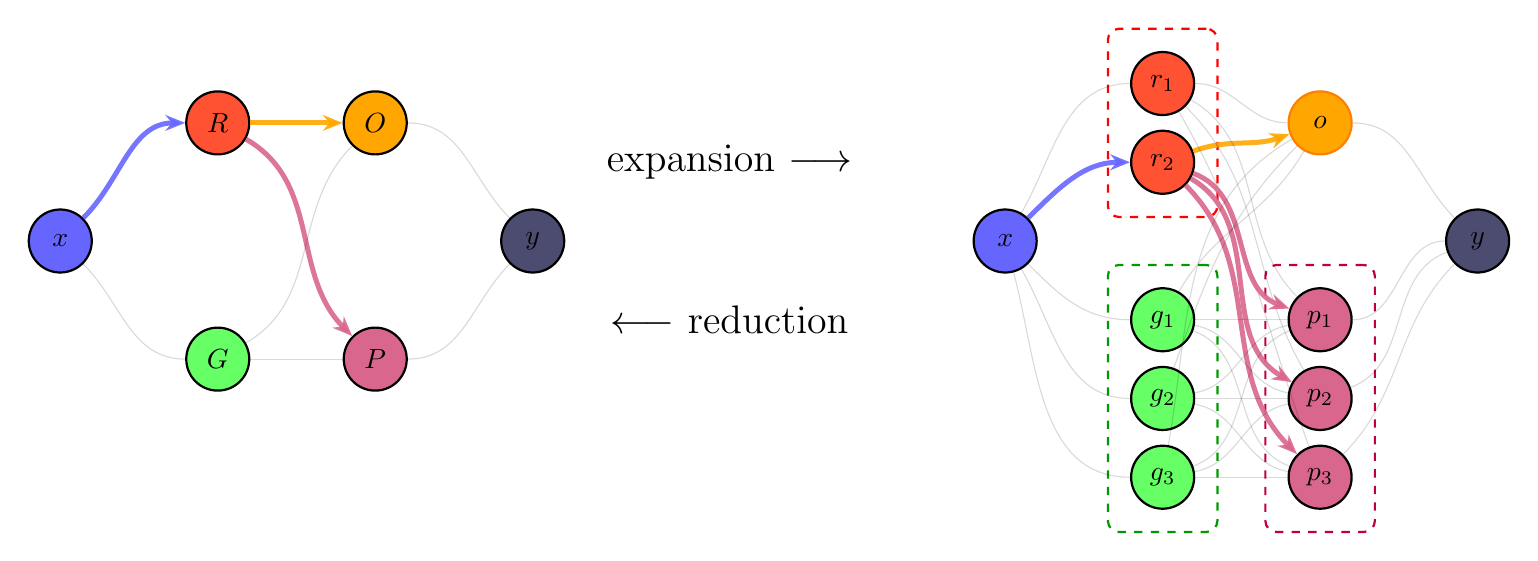
\begin{tikzpicture}[
    node/.style={circle, draw, minimum size=0.8cm, thick},
    xnode/.style={node, fill=blue!60},
    ynode/.style={node, fill=blue!20!black!70},
    rnode/.style={node, fill=red!70!orange!80},
    gnode/.style={node, fill=green!60},
    onode/.style={node, fill=orange!70!yellow},
    pnode/.style={node, fill=purple!60},
    % Edge styles
    faintedge/.style={black, opacity=0.15, thin},
    redge/.style={red!70!orange!80, opacity=0.9, line width=1.8pt, -{Stealth[length=2.5mm, width=2mm]}},
    gedge/.style={green!60, opacity=0.9, line width=1.8pt, -{Stealth[length=2.5mm, width=2mm]}},
    oedge/.style={orange!70!yellow, opacity=0.9, line width=1.8pt, -{Stealth[length=2.5mm, width=2mm]}},
    pedge/.style={purple!60, opacity=0.9, line width=1.8pt, -{Stealth[length=2.5mm, width=2mm]}},
    blueedge/.style={blue!60, opacity=0.9, line width=1.8pt, -{Stealth[length=2.5mm, width=2mm]}},
    arrow/.style={-{Latex[length=3mm]}, line width=3pt, gray!80},
    ]
    
    % Left network (simplified) with updated labels
    \node[xnode] (x1) at (0,0) {$x$};
    \node[rnode] (hr1) at (2,1.5) {$R$};
    \node[gnode] (hg1) at (2,-1.5) {$G$};
    \node[onode] (ho1) at (4,1.5) {$O$};
    \node[pnode] (hp1) at (4,-1.5) {$P$};
    \node[ynode] (y1) at (6,0) {$y$};
    
    % Connections for left network - all faint except those to/from hr1
    % x to hr1 (highlighted with arrow)
    \draw[blueedge] (x1) to[out=45, in=180] (hr1);
    % x to hg1 (faint)
    \draw[faintedge] (x1) to[out=-45, in=180] (hg1);
    % hr1 to ho1 (highlighted with arrow)
    \draw[oedge] (hr1) to[out=0, in=180] (ho1);
    % hr1 to hp1 (highlighted with arrow)
    \draw[pedge] (hr1) to[out=-30, in=135] (hp1);
    % hg1 to ho1 (faint)
    \draw[faintedge] (hg1) to[out=30, in=-135] (ho1);
    % hg1 to hp1 (faint)
    \draw[faintedge] (hg1) to[out=0, in=180] (hp1);
    % ho1 to y1 (faint)
    \draw[faintedge] (ho1) to[out=0, in=135] (y1);
    % hp1 to y1 (faint)
    \draw[faintedge] (hp1) to[out=0, in=-135] (y1);
    
    % Right network (expanded) - shifted horizontally with updated labels
    \node[xnode] (x2) at (12,0) {$x$};
    
    % Create multiple nodes for each color in the expanded network
    \node[rnode] (hr2_1) at (14,2) {$r_1$};
    \node[rnode] (hr2_2) at (14,1) {$r_2$};
    
    \node[gnode] (hg2_1) at (14,-1) {$g_1$};
    \node[gnode] (hg2_2) at (14,-2) {$g_2$};
    \node[gnode] (hg2_3) at (14,-3) {$g_3$};
    
    \node[onode, draw=orange, thick] (ho2) at (16,1.5) {$o$};
    
    \node[pnode] (hp2_1) at (16,-1) {$p_1$};
    \node[pnode] (hp2_2) at (16,-2) {$p_2$};
    \node[pnode] (hp2_3) at (16,-3) {$p_3$};
    
    \node[ynode] (y2) at (18,0) {$y$};
    
    % Connections from x to all red and green nodes
    \draw[faintedge] (x2) to[out=60, in=180] (hr2_1);
    \draw[blueedge] (x2) to[out=45, in=180] (hr2_2); % Highlighted with arrow
    \draw[faintedge] (x2) to[out=-45, in=180] (hg2_1);
    \draw[faintedge] (x2) to[out=-60, in=180] (hg2_2);
    \draw[faintedge] (x2) to[out=-75, in=180] (hg2_3);
    
    % Connections from all red nodes to orange node
    \draw[faintedge] (hr2_1) to[out=0, in=180] (ho2);
    \draw[oedge] (hr2_2) to[out=20, in=200] (ho2); % Highlighted with arrow
    
    % Connections from all red nodes to all purple nodes
    \draw[faintedge] (hr2_1) to[out=-30, in=135] (hp2_1);
    \draw[faintedge] (hr2_1) to[out=-45, in=120] (hp2_2);
    \draw[faintedge] (hr2_1) to[out=-60, in=110] (hp2_3);
    
    \draw[pedge] (hr2_2) to[out=-20, in=160] (hp2_1); % Highlighted with arrow
    \draw[pedge] (hr2_2) to[out=-30, in=150] (hp2_2); % Highlighted with arrow
    \draw[pedge] (hr2_2) to[out=-45, in=135] (hp2_3); % Highlighted with arrow
    
    % Connections from all green nodes to orange node
    \draw[faintedge] (hg2_1) to[out=60, in=-120] (ho2);
    \draw[faintedge] (hg2_2) to[out=70, in=-135] (ho2);
    \draw[faintedge] (hg2_3) to[out=80, in=-150] (ho2);
    
    % Connections from all green nodes to all purple nodes
    % All faint as they don't connect to hr2_2
    \draw[faintedge] (hg2_1) to[out=0, in=180] (hp2_1);
    \draw[faintedge] (hg2_1) to[out=-10, in=170] (hp2_2);
    \draw[faintedge] (hg2_1) to[out=-20, in=160] (hp2_3);
    
    \draw[faintedge] (hg2_2) to[out=10, in=190] (hp2_1);
    \draw[faintedge] (hg2_2) to[out=0, in=180] (hp2_2);
    \draw[faintedge] (hg2_2) to[out=-10, in=170] (hp2_3);
    
    \draw[faintedge] (hg2_3) to[out=20, in=200] (hp2_1);
    \draw[faintedge] (hg2_3) to[out=10, in=190] (hp2_2);
    \draw[faintedge] (hg2_3) to[out=0, in=180] (hp2_3);
    
    % Connections from orange to y (faint since not directly from hr2_2)
    \draw[faintedge] (ho2) to[out=0, in=135] (y2);
    
    % Connections from all purple nodes to y (faint since not directly from hr2_2)
    \draw[faintedge] (hp2_1) to[out=0, in=180] (y2);
    \draw[faintedge] (hp2_2) to[out=20, in=-160] (y2);
    \draw[faintedge] (hp2_3) to[out=45, in=-135] (y2);
    
    % Add dashed outlines around groups
    \begin{pgfonlayer}{background}
        \node[draw=red, dashed, thick, rounded corners, fit=(hr2_1) (hr2_2), inner sep=8pt] {};
        \node[draw=green!60!black, dashed, thick, rounded corners, fit=(hg2_1) (hg2_2) (hg2_3), inner sep=8pt] {};
        \node[draw=purple, dashed, thick, rounded corners, fit=(hp2_1) (hp2_2) (hp2_3), inner sep=8pt] {};
    \end{pgfonlayer}
    
    % Add horizontal arrows for reduction and expansion
    \node at (8.5,1) {\Large expansion $\longrightarrow$};
    \node at (8.5,-1) {\Large $\longleftarrow$ reduction};
    
\end{tikzpicture}
}
% \end{figure}

\begin{figure}[t]
    \centering
    \resizebox{\textwidth}{!}{
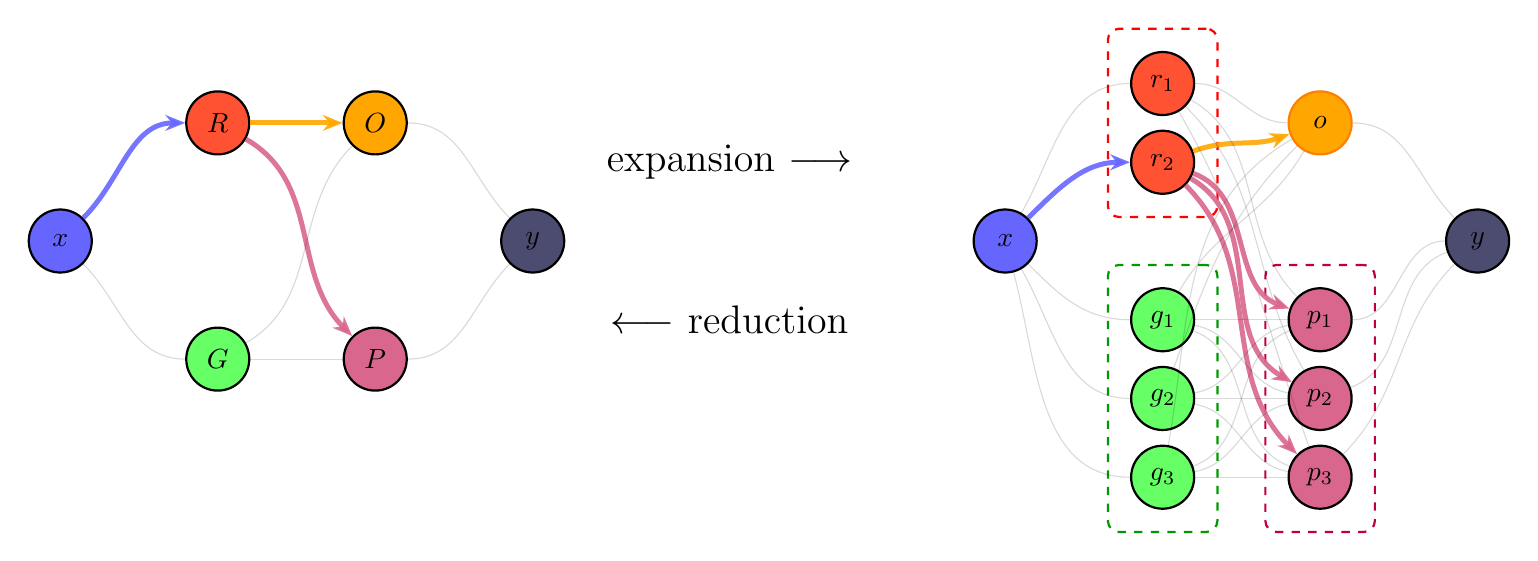
\begin{tikzpicture}[
    node/.style={circle, draw, minimum size=0.8cm, thick},
    xnode/.style={node, fill=blue!60},
    ynode/.style={node, fill=blue!20!black!70},
    rnode/.style={node, fill=red!70!orange!80},
    gnode/.style={node, fill=green!60},
    onode/.style={node, fill=orange!70!yellow},
    pnode/.style={node, fill=purple!60},
    % Edge styles
    faintedge/.style={black, opacity=0.15, thin},
    redge/.style={red!70!orange!80, opacity=0.9, line width=1.8pt, -{Stealth[length=2.5mm, width=2mm]}},
    gedge/.style={green!60, opacity=0.9, line width=1.8pt, -{Stealth[length=2.5mm, width=2mm]}},
    oedge/.style={orange!70!yellow, opacity=0.9, line width=1.8pt, -{Stealth[length=2.5mm, width=2mm]}},
    pedge/.style={purple!60, opacity=0.9, line width=1.8pt, -{Stealth[length=2.5mm, width=2mm]}},
    blueedge/.style={blue!60, opacity=0.9, line width=1.8pt, -{Stealth[length=2.5mm, width=2mm]}},
    arrow/.style={-{Latex[length=3mm]}, line width=3pt, gray!80},
    ]
    
    % Left network (simplified) with updated labels
    \node[xnode] (x1) at (0,0) {$x$};
    \node[rnode] (hr1) at (2,1.5) {$R$};
    \node[gnode] (hg1) at (2,-1.5) {$G$};
    \node[onode] (ho1) at (4,1.5) {$O$};
    \node[pnode] (hp1) at (4,-1.5) {$P$};
    \node[ynode] (y1) at (6,0) {$y$};
    
    % Connections for left network - all faint except those to/from hr1
    % x to hr1 (highlighted with arrow)
    \draw[blueedge] (x1) to[out=45, in=180] (hr1);
    % x to hg1 (faint)
    \draw[faintedge] (x1) to[out=-45, in=180] (hg1);
    % hr1 to ho1 (highlighted with arrow)
    \draw[oedge] (hr1) to[out=0, in=180] (ho1);
    % hr1 to hp1 (highlighted with arrow)
    \draw[pedge] (hr1) to[out=-30, in=135] (hp1);
    % hg1 to ho1 (faint)
    \draw[faintedge] (hg1) to[out=30, in=-135] (ho1);
    % hg1 to hp1 (faint)
    \draw[faintedge] (hg1) to[out=0, in=180] (hp1);
    % ho1 to y1 (faint)
    \draw[faintedge] (ho1) to[out=0, in=135] (y1);
    % hp1 to y1 (faint)
    \draw[faintedge] (hp1) to[out=0, in=-135] (y1);
    
    % Right network (expanded) - shifted horizontally with updated labels
    \node[xnode] (x2) at (12,0) {$x$};
    
    % Create multiple nodes for each color in the expanded network
    \node[rnode] (hr2_1) at (14,2) {$r_1$};
    \node[rnode] (hr2_2) at (14,1) {$r_2$};
    
    \node[gnode] (hg2_1) at (14,-1) {$g_1$};
    \node[gnode] (hg2_2) at (14,-2) {$g_2$};
    \node[gnode] (hg2_3) at (14,-3) {$g_3$};
    
    \node[onode, draw=orange, thick] (ho2) at (16,1.5) {$o$};
    
    \node[pnode] (hp2_1) at (16,-1) {$p_1$};
    \node[pnode] (hp2_2) at (16,-2) {$p_2$};
    \node[pnode] (hp2_3) at (16,-3) {$p_3$};
    
    \node[ynode] (y2) at (18,0) {$y$};
    
    % Connections from x to all red and green nodes
    \draw[faintedge] (x2) to[out=60, in=180] (hr2_1);
    \draw[blueedge] (x2) to[out=45, in=180] (hr2_2); % Highlighted with arrow
    \draw[faintedge] (x2) to[out=-45, in=180] (hg2_1);
    \draw[faintedge] (x2) to[out=-60, in=180] (hg2_2);
    \draw[faintedge] (x2) to[out=-75, in=180] (hg2_3);
    
    % Connections from all red nodes to orange node
    \draw[faintedge] (hr2_1) to[out=0, in=180] (ho2);
    \draw[oedge] (hr2_2) to[out=20, in=200] (ho2); % Highlighted with arrow
    
    % Connections from all red nodes to all purple nodes
    \draw[faintedge] (hr2_1) to[out=-30, in=135] (hp2_1);
    \draw[faintedge] (hr2_1) to[out=-45, in=120] (hp2_2);
    \draw[faintedge] (hr2_1) to[out=-60, in=110] (hp2_3);
    
    \draw[pedge] (hr2_2) to[out=-20, in=160] (hp2_1); % Highlighted with arrow
    \draw[pedge] (hr2_2) to[out=-30, in=150] (hp2_2); % Highlighted with arrow
    \draw[pedge] (hr2_2) to[out=-45, in=135] (hp2_3); % Highlighted with arrow
    
    % Connections from all green nodes to orange node
    \draw[faintedge] (hg2_1) to[out=60, in=-120] (ho2);
    \draw[faintedge] (hg2_2) to[out=70, in=-135] (ho2);
    \draw[faintedge] (hg2_3) to[out=80, in=-150] (ho2);
    
    % Connections from all green nodes to all purple nodes
    % All faint as they don't connect to hr2_2
    \draw[faintedge] (hg2_1) to[out=0, in=180] (hp2_1);
    \draw[faintedge] (hg2_1) to[out=-10, in=170] (hp2_2);
    \draw[faintedge] (hg2_1) to[out=-20, in=160] (hp2_3);
    
    \draw[faintedge] (hg2_2) to[out=10, in=190] (hp2_1);
    \draw[faintedge] (hg2_2) to[out=0, in=180] (hp2_2);
    \draw[faintedge] (hg2_2) to[out=-10, in=170] (hp2_3);
    
    \draw[faintedge] (hg2_3) to[out=20, in=200] (hp2_1);
    \draw[faintedge] (hg2_3) to[out=10, in=190] (hp2_2);
    \draw[faintedge] (hg2_3) to[out=0, in=180] (hp2_3);
    
    % Connections from orange to y (faint since not directly from hr2_2)
    \draw[faintedge] (ho2) to[out=0, in=135] (y2);
    
    % Connections from all purple nodes to y (faint since not directly from hr2_2)
    \draw[faintedge] (hp2_1) to[out=0, in=180] (y2);
    \draw[faintedge] (hp2_2) to[out=20, in=-160] (y2);
    \draw[faintedge] (hp2_3) to[out=45, in=-135] (y2);
    
    % Add dashed outlines around groups
    \begin{pgfonlayer}{background}
        \node[draw=red, dashed, thick, rounded corners, fit=(hr2_1) (hr2_2), inner sep=8pt] {};
        \node[draw=green!60!black, dashed, thick, rounded corners, fit=(hg2_1) (hg2_2) (hg2_3), inner sep=8pt] {};
        \node[draw=purple, dashed, thick, rounded corners, fit=(hp2_1) (hp2_2) (hp2_3), inner sep=8pt] {};
    \end{pgfonlayer}
    
    % Add horizontal arrows for reduction and expansion
    \node at (8.5,1) {\Large expansion $\longrightarrow$};
    \node at (8.5,-1) {\Large $\longleftarrow$ reduction};
    
\end{tikzpicture}
}
    \caption{Illustration of network expansion and reduction according to Proposition~\ref{prop:cloned}.}
    \label{fig:plasticity-manifolds}
\end{figure}


\begin{remark}
The sub‑space in Proposition~\ref{prop:cloned} is a stable manifold for any gradient‑based optimiser that relies solely on first‑order statistics (SGD, momentum, Adam) and for any data distribution.
\end{remark}

\section{Mitigating and recovering plasticity}
\label{sec:mitigate}

\subsection{Rank preservation via nonlinearities and Gaussianity}

\begin{proposition}[Rank preservation lemma]
\label{prop:rank}
Let $f:\R\to\R$ be square‑integrable w.r.t.\ $\mathcal{N}(0,1)$ and not a bounded‑degree polynomial.  
If pre‑activations $z\in\R^d$ are jointly Gaussian with $\E z_i z_j=\rho_{ij}$ and $|\rho_{ij}|<1$, then the post‑activation covariance $C=\E[f(z)f(z)^\top]$ is full rank except when two features are exact duplicates.
\end{proposition}

\paragraph{Design implications.}
BatchNorm (which Gaussianises pre‑activations) and dropout (which breaks symmetry) combat rank collapse, thereby delaying loss of plasticity.

\subsection{Escaping a plasticity‑loss manifold}

\begin{corollary}[Perturbation dynamics]
\label{cor:perturb}
Let $\theta_0\in\mathcal{M}$ and perturb along $v\in N_{\theta_0}\mathcal{M}$, $\|v\|=1$:
\[
\theta(0)=\theta_0+\varepsilon v,\qquad \varepsilon\ll1.
\]
Then
\(
\frac{d}{dt}\bigl.\mathrm{dist}^2(\theta(t),\mathcal{M})\bigr|_{t=0}
=-2\varepsilon\,v^\top\nabla_\theta^2\Loss(\theta_0)v+O(\varepsilon^2).
\)
Plasticity is recovered (distance grows) iff some normal direction has negative curvature, explaining why noise injections or re‑initialisation occasionally succeed.
\end{corollary}

\section{Empirical Evaluation (in progress)}
\label{sec:experiments}

The empirical evidence will be supporting the key hypothesis in this manuscript 
\begin{itemize}
    \item Emergence of frozen and duplicate units is a as a result of prolonged training, which will lead  to loss of plasticity 
    \item The cloning hypothesis: if we create a cloned model, it will remain constrained to the smaller model sub-space.
    \item Escaping cloned sub-space: if the model has dropout, or if we inject some noise into the back propagation, it will escape the sub-space 
\end{itemize}

\section{Discussion and open questions}
Our analysis casts several well‑known empirical phenomena—dead ReLUs, neural collapse, weight duplication—into a common dynamical framework. It raises new questions:
\begin{itemize}[nosep]
    \item Can we design \emph{continual} randomisation schemes that keep trajectories away from stable plasticity‑loss manifolds?
    \item How do second‑order or meta‑gradient methods interact with the manifolds identified here?
    \item Is there a loss of plasticity of non-linear form, ie, where the sub-space is not linear? 
    \item Can plasticity be preserved in parameter‑efficient fine‑tuning (LoRA, adapters) by ensuring adapter sub‑spaces do not themselves collapse?
\end{itemize}
We leave these directions to future work.

\section{Broader Impacts}
This work contributes to understanding fundamental limitations in continual learning systems. Positive societal impacts include more robust AI systems that can adapt to changing environments without degradation, potentially leading to more reliable autonomous systems and reduced need for frequent retraining. Negative impacts might include enabling systems that continue to adapt in unpredictable ways if deployed without proper safeguards. Our theoretical framework provides tools to better understand and potentially mitigate these risks.

\bibliographystyle{plain}
\bibliography{paper/refs}

\appendix 
\section{Proofs}
\label{app:proofs}

\begin{proof}[Proof of proposition on cloning loss of plasticity]
    \textbf{Forward cloning.} First we prove that for any input $x \in \R^{|V_{in}|},$ any node in each partition will have similar values:
    \begin{align*}
        \forall S \in \{S_1,\dots,S_{|V|}\} \implies \forall u,v \in S, h(u) = h(v). 
    \end{align*}
    We do so by induction over the directed distance from inputs:
    Suppose that for all nodes where $dist(V_{in},v) \le i$ in the larger graph, we have that $h(v)$ is constant across each partition: 
    \begin{align*}
        &T_i:= \{v\in \mathcal{V}: dist(V_{in},v) \le i\} && \text{nodes $i$-steps from input}\\
        &\forall S \in \{S_1,\dots,S_{|V|}\}, \; \forall u,v \in (S\cap T_i): h(v) = h(u)  && \text{induction hypothesis}
    \end{align*}
    First, note that the induction is trivially valid for $i=0,$ because inputs in the larger and smaller model coincide. 
    For some partition $S$, consider all nodes $v \in S$ whose distance from the input is $dist(\mathcal{V}_{in},v) \le i+1.$ Then, by the induction hypothesis know that all their incoming units in the same partition will have a similar value. Furthermore, because of the incoming weight condition, we know that the sum of incoming weights from each partition is similar for all these units. Thus, their weights are essentially a re-distribution between units with similar values and thus make no difference. As a result, their values will also be identical, which proves the induction step. Thus, we have proven the forward cloning of the units. 
    
    \textbf{Backward cloning.} We now prove a very similar result but for the backward $\delta(v)$ of all units:
        \begin{align*}
        \forall S \in \{S_1,\dots,S_{|V|}\} \implies \forall u,v \in S, \delta(u) = \delta(v). 
    \end{align*}
    We prove this similar to forward, but the induction is defined as steps from the output. In other words, we prove it first for the output nodes, and then prove it for nodes that are 1,2,... steps away from it: 
        \begin{align*}
        &T_i:= \{v\in \mathcal{V}: dist(v,V_{in}) \le i\} && \text{nodes $i$-steps from input}\\
        &\forall S \in \{S_1,\dots,S_{|V|}\}, \; \forall u,v \in (S\cap T_i): \delta(v) = \delta(u)  && \text{induction hypothesis}
    \end{align*}
    Again, this is trivially true for $i=0,$ because output units are coinciding between the two networks, and we have already established that the forward pass values are similar for these units in the forward cloning step. Thus, the backward errors of the output units will also be cloned. Now, suppose that we have the induction hypothesis for $i,$ and want to prove it for $i+1.$ Consider units $u,v$ in some partition $S,$ that are at most $i+1$ steps away from the output units. By induction hypothesis, all their outgoing units will be cloned, i.e., have similar values across each partition. Now, given the outgoing weight condition, the sum of the weights to each outgoing partition is equal for $u,v.$ Thus, we can view their outgoing weights as redistributing weights between units in same partition. Because by induction hypothesis these units have similar backward values, this redistribution of weights will not change the value of the unit, and thus, we will always have $\delta(v) = \delta(u),$ which proves the induction step.

    \textbf{Weight gradient cloning.} Now that we have proven forward and backward cloning, we can easily prove that given two partitions $S, S',$ any two units from these partitions will have similar weight gradients:
    \begin{align*}
        S,S' \in \{S_1,\dots, S_{|V|}\} \text{ then } \forall u,u' \in S, v,v'\in S': \frac{\partial \Loss}{\partial W(u,v)}=\frac{\partial \Loss}{\partial W(u',v')}.
    \end{align*}
    In other words, the gradient of weights between any units in two partitions will be constant across partitions. More importantly, applying this gradient step will not violate the forward and backward symmetry conditions, and thus the next steps will also have similar gradients. Because these gradients have block-wise structure determined by the partition, and change from initialization can be described a by a weight matrix $W(S_u,S_v)$ whose dimensions is only the number of edges between the partitions $|E|$ rather than the original model $|\mathcal{E}|$. Furthermore, this lower-dimensional manifold can be described as an affine sub-space int he space of all possible parametres. 
\end{proof}

\begin{proof}[Proof of rank preservation proposition]
Because $f$ is square-integrable, it has an infinite Hermite expansion $f(z)=\sum_{k=0}^{\infty} b_k\, \He_k(z)$. Mehler's formula implies that $\mathbb{E}[\He_k(x_i)\He_\ell(x_j)]$ vanishes unless $k=\ell$, in which case it scales like $C_{ij}^k$. Summing across $k$, we get 
\begin{align*}
\mathbb{E}[f(x_i)f(x_j)] 
= 
\sum_{k=0}^{\infty} b_k^2\,C_{ij}^k.
\end{align*}
Since $b_k\neq 0$ for infinitely many $k$, and $|C_{ij}|<1$, eventually the Hadamard powers $C^{\odot k}$ are strictly positive semidefinite (by Gershgorin arguments), forcing the resulting sum to be positive definite. Thus, $M$ is full-rank.
\end{proof}

\section{Corollary on architectural extensions}
\begin{itemize}
    \item Bias: we can add bias to the linear units by augmenting the input units with an always $1$ unit, and then adding an edge between this input unit and any unit that needs a bias. Because bias is just like a weight times $1$ unit. 
    \item CNN: while the proposition resembles the definition of an MLP unit, the channels in a CNN module can be effectively viewed as a single unit: in fact, we can view each channel as application of a MLP unit on various patches of the input channels. Thus, in the CNN context, we can form and define the equivalences between channels as opposed to neurons in a MLP. 
    \item Softmax/RMSNorm/LayerNorm layers: in the proposition, the definition of each unit only allows for linear and element-wise activation units. This does not include units that rely non-linearly on a number of features is not be directly covered under the current proposition. For this type of modules, we can create an ad-hoc low-dimensional alternative that is aware of the multiplicity of the duplicated units. More specifically, if a unit takes $n$-dimensional input, and these input features are divided into $m$ partitions: $S_1\dot\cup \dots \dot S_m = \{1,\dots, n\}, $ then we can define the low dimensional counter-part, for example for LayerNorm  we have  
    \begin{align*}
        \text{low-dim-LN}(x)_i = \frac{(x_i-\mu(x))}{\sqrt{var(x)}} \quad 
        \mu(x) = \sum_{i\le m} |S_i| h_m, \quad var(x) =\sum_{i\le m} |S_i| (h_i-\mu_i )^2
    \end{align*}
    where $h_i$ is the value of the input partition $S_i$
    and for softmax we have
    \begin{align*}
        \text{low-dim-Softmax}(x) = \frac{e^{x_i}}{\sum_{j\le m} |S_j| e^{h_j}}
    \end{align*}
    where $h_j$ is the value of the input partition $S_j$.
\end{itemize}

We can also extend the proposition in terms of optimization algorithm:
\begin{itemize}
    \item SGD with mini-batch gradients: while the definition of the proposition is stated for a single sample, adding multiple sample gradients will be simply the sum of multiple gradients that has the cloning structure. And because addition will preserve the weight cloning structure, the gradients of a SGD optimization will not alter the results. 
    \item SGD with momentum/ Adam: While the statement was given for a vanilla gradient, any subsequent gradient statistics such as momentum or Adam stats will also follow a similar cloning structure, and thus, using momentum or Adam will not alter the results.  
\end{itemize}

\section*{NeurIPS Paper Checklist}
\begin{enumerate}
\item {\bf Claims}
    \item[] Answer: \answerYes{} 
    \item[] Justification: The claims in the abstract and introduction accurately reflect the paper's contributions on loss of plasticity in neural networks.

\item {\bf Limitations}
    \item[] Answer: \answerYes{} 
    \item[] Justification: Limitations are discussed in the Discussion section, acknowledging open questions and future work.

\item {\bf Theory assumptions and proofs}
    \item[] Answer: \answerYes{} 
    \item[] Justification: All theoretical results include assumptions and complete proofs are provided in the appendix.
    
\item {\bf Experimental result reproducibility}
    \item[] Answer: \answerYes{} 
    \item[] Justification: The paper provides detailed experimental settings, benchmarks, and protocols in Section 5.

\item {\bf Open access to data and code}
    \item[] Answer: \answerYes{} 
    \item[] Justification: Code and data will be made available upon acceptance.

\item {\bf Experimental setting/details}
    \item[] Answer: \answerYes{} 
    \item[] Justification: The paper details architectures, variants, optimizers, and training protocols in Section 5.

\item {\bf Experiment statistical significance}
    \item[] Answer: \answerYes{} 
    \item[] Justification: The paper describes methods for statistical evaluation in the Metrics section.

\item {\bf Experiments compute resources}
    \item[] Answer: \answerNo{} 
    \item[] Justification: We will add details about compute resources (GPUs, memory, training time) in the final version.

\item {\bf Code of ethics}
    \item[] Answer: \answerYes{} 
    \item[] Justification: The research conforms to the NeurIPS Code of Ethics.

\item {\bf Broader impacts}
    \item[] Answer: \answerYes{} 
    \item[] Justification: The paper discusses both positive impacts (more robust adaptive systems) and potential negative ones (unpredictable adaptation).

\item {\bf Safeguards}
    \item[] Answer: \answerNA{} 
    \item[] Justification: This paper is theoretical and does not release models or datasets with high risk for misuse.

\item {\bf Licenses for existing assets}
    \item[] Answer: \answerYes{} 
    \item[] Justification: All datasets used (CIFAR-100, MNIST) are publicly available with standard licenses.

\item {\bf New assets}
    \item[] Answer: \answerYes{} 
    \item[] Justification: Code and experiment configurations will be well-documented upon release.

\item {\bf Crowdsourcing and research with human subjects}
    \item[] Answer: \answerNA{} 
    \item[] Justification: This research does not involve human subjects or crowdsourcing.

\item {\bf Institutional review board (IRB) approvals or equivalent for research with human subjects}
    \item[] Answer: \answerNA{} 
    \item[] Justification: This research does not involve human subjects.

\item {\bf Declaration of LLM usage}
    \item[] Answer: \answerNA{} 
    \item[] Justification: No LLMs were used in the development of the core methods in this research.
\end{enumerate}
\end{document}